\subsection{Two computational routes}

Let $A=J+E$ denote the guarded operand in one fixed reference contract.
The exact parent and response problems are
\begin{linenomath*}
\begin{equation}
Jz=b,\qquad Az_g=b,\qquad A\delta z=-Ez,
\qquad \delta z=z_g-z.
\label{eq:route_exact_problems}
\end{equation}
\end{linenomath*}
Here $E=A-J$ is the realized perturbation of the two solve operands. The
declared $\Delta J$ remains the operand used by the floating-point
forcing construction. This distinction is immaterial when addition is exact,
but retains last-bit operand effects when $A$ and $J$ are captured
independently under IEEE~754 binary arithmetic \cite{S09,S10}.

The direct route computes two parent solutions and subtracts them,
\begin{linenomath*}
\begin{equation}
\widetilde\delta_{\rm d}
=\operatorname{fl}(\widetilde z_g-\widetilde z)
=\delta z+e_g-e+q_{\rm sub},
\label{eq:direct_operation_graph}
\end{equation}
\end{linenomath*}
where $e=\widetilde z-z$, $e_g=\widetilde z_g-z_g$, and
$q_{\rm sub}$ is the subtraction error.

\begin{proposition}[Direct-difference error enclosure]
\label{prop:p4}
If $\lVert e\rVert_2\leq U_z$,
$\lVert e_g\rVert_2\leq U_{z_g}$, and
$\lVert q_{\rm sub}\rVert_2\leq U_{\rm sub}$, then
\begin{linenomath*}
\begin{equation}
\lVert\widetilde\delta_{\rm d}-\delta z\rVert_2
\leq U_{\rm d}:=U_z+U_{z_g}+U_{\rm sub}.
\label{eq:direct_difference_enclosure}
\end{equation}
\end{linenomath*}
\end{proposition}

\begin{proof}
Subtract $\delta z$ from Eq.~\eqref{eq:direct_operation_graph} and apply
the triangle inequality.
\end{proof}

The response route constructs
$\widetilde f=\operatorname{fl}(-\Delta J\widetilde z)$ and solves
$A\widetilde\delta_{\rm r}\approx\widetilde f$. Define the forcing
defect $q_f=\widetilde f+E\widetilde z$ and response residual
$r_\delta=\widetilde f-A\widetilde\delta_{\rm r}$.

\begin{proposition}[Response-equation error enclosure]
\label{prop:p5}
Assume $\lVert\widetilde z-z\rVert_2\leq U_z$ and let
$\beta_A\geq\lVert A^{-1}\rVert_2$ and
$\alpha_E\geq\lVert E\rVert_2$. Then
\begin{linenomath*}
\begin{equation}
\begin{aligned}
\lVert\widetilde\delta_{\rm r}-\delta z\rVert_2
&\leq U_{\rm r},\\
U_{\rm r}
&:=\underbrace{\beta_A\alpha_EU_z}_{U_{\rm parent}}
+\underbrace{\beta_A\lVert q_f\rVert_2}_{U_{\rm force}}
+\underbrace{\beta_A\lVert r_\delta\rVert_2}_{U_{\rm solve}}.
\end{aligned}
\label{eq:response_equation_enclosure}
\end{equation}
\end{linenomath*}
\end{proposition}

\begin{proof}
Because $A\delta z=-Ez$ and
$A\widetilde\delta_{\rm r}=\widetilde f-r_\delta$,
\[
A(\widetilde\delta_{\rm r}-\delta z)
=q_f-E(\widetilde z-z)-r_\delta .
\]
Multiplication by $A^{-1}$, submultiplicativity, and the assumed majorants
give Eq.~\eqref{eq:response_equation_enclosure}.
\end{proof}

Propositions~\ref{prop:p4} and \ref{prop:p5} enclose the same exact
response through different operation graphs. Their components therefore
cannot be exchanged merely because the observed response vectors are close.

\subsection{Parent bounds, threshold relation, and reference contracts}

For a computed solution $\widetilde x$ of $Bx=c$, residual
$r=c-B\widetilde x$, and any
$\beta_B\geq\lVert B^{-1}\rVert_2$, the parent error satisfies
\begin{linenomath*}
\begin{equation}
\lVert\widetilde x-x\rVert_2
\leq\lVert B^{-1}\rVert_2\lVert r\rVert_2
\leq\beta_B\lVert r\rVert_2.
\label{eq:parent_majorant}
\end{equation}
\end{linenomath*}
The implementation uses
\begin{linenomath*}
\begin{equation}
\beta_B=\lVert B^{-1}\rVert_F\geq\lVert B^{-1}\rVert_2,
\qquad
\alpha_E=\lVert E\rVert_F\geq\lVert E\rVert_2.
\label{eq:frobenius_majorants}
\end{equation}
\end{linenomath*}
Thus the Frobenius quantities are explicit majorants; they are not
subordinate matrix norms paired with the Euclidean vector norm.
For binary64 subtraction, the adopted allowance is
\begin{linenomath*}
\begin{equation}
U_{\rm sub}
=\gamma_1\lVert|\widetilde z_g|+|\widetilde z|\rVert_2
+\sqrt n\,2^{-1075},\qquad
\gamma_1=\frac{2^{-53}}{1-2^{-53}}.
\label{eq:subtraction_allowance}
\end{equation}
\end{linenomath*}

For either route $a\in\{\mathrm d,\mathrm r\}$, let
$d_a=\lVert\widetilde\delta_a\rVert_2$ and let $U_a$ be the matching
enclosure. The response-magnitude interval is
\begin{linenomath*}
\begin{equation}
L_a=\max(0,d_a-U_a),\qquad H_a=d_a+U_a.
\label{eq:response_magnitude_interval}
\end{equation}
\end{linenomath*}

\begin{corollary}[Sound threshold relation]
\label{cor:threshold}
If Proposition~\ref{prop:p4} or \ref{prop:p5} applies, then
$L_a\leq\lVert\delta z\rVert_2\leq H_a$. Hence, for a threshold
$\tau\geq0$ fixed independently of the observed response,
$L_a>\tau$ proves that the exact response exceeds $\tau$, and
$H_a<\tau$ proves that it lies below $\tau$.
\end{corollary}

\begin{definition}[Route-qualified threshold relation]
The outcome is \emph{above} if $L_a>\tau$, \emph{below} if
$H_a<\tau$, and \emph{unresolved} otherwise. Setting $\tau=0$ recovers
zero exclusion as a special case.
\end{definition}

Two reference contracts are retained. The decimal-source contract treats the
registered decimal matrices and vectors as the real-valued problem. The
binary64-operand contract reconstructs the captured IEEE operands exactly and
treats those values as a separate real-valued problem. Each residual,
inverse majorant, forcing defect, and reference response is evaluated only
within its matching contract. Figure~\ref{fig:5} shows both reference lanes
and both operation graphs.

\begin{figure}[H]
\centering
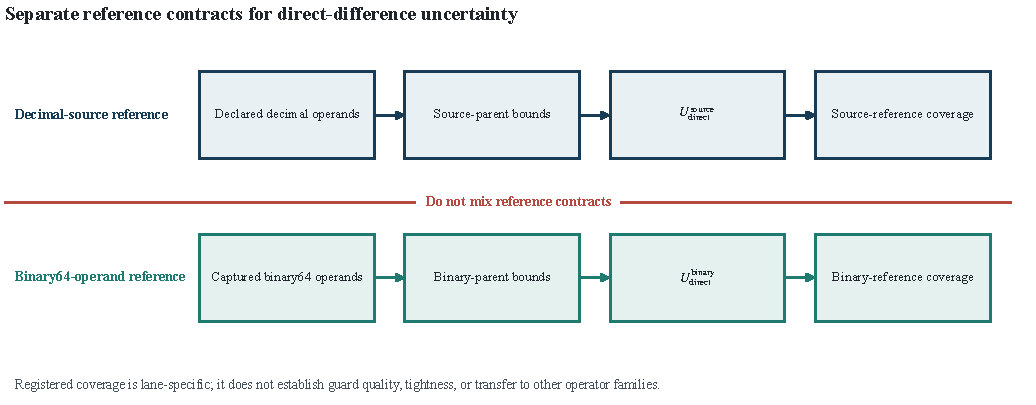
\includegraphics[width=0.98\linewidth,height=0.72\textheight,keepaspectratio]{F5_two_reference_contracts.pdf}
\caption{Reference-contract and operation-graph anatomy. Decimal-source and binary64-operand problems remain separate. Within either contract, direct subtraction combines two parent and subtraction components, whereas the response equation combines parent propagation, forcing construction, and response-solve components.}
\label{fig:5}
\end{figure}

\subsection{Prospective enclosure validation}

The direct-route model was first evaluated on a 300-system development set
and a disjoint 300-system holdout containing SPD, nonsymmetric, and
saddle-point-like matrices of dimensions $2$, $4$, $8$, and $16$. Each
reference contract achieved 300/300 coverage on both sets. A subsequent
preregistered response-route study froze Proposition~\ref{prop:p5} and then
generated a new 300-system holdout with disjoint seeds, condition exponents,
and perturbation amplitudes. Both routes were evaluated without changing the
matrices or gates.

Table~\ref{tab:routevalidation} reports the result. Direct and response
enclosures each covered 300/300 errors in all four data-set--contract
combinations. The development decimal-source response error was lower in
295/300 cases, reproducing the earlier route comparison; the corresponding
count was 271/300 on the new holdout. In the binary64-operand contract, the
counts were 199/300 and 160/300. Lower response error therefore did not imply
a universal route ordering.

\begin{table}[htbp]
\centering
\footnotesize
\caption{Prospective direct- and response-route enclosure validation. Coverage is shown as covered/total; the last two columns count cases in which the response route produced the smaller quantity.}
\label{tab:routevalidation}
\begin{tabularx}{\linewidth}{>{\RaggedRight\arraybackslash}p{0.16\linewidth} >{\RaggedRight\arraybackslash}p{0.16\linewidth} *{4}{>{\centering\arraybackslash}X}}
\toprule
Set & Reference contract & Direct coverage & Response coverage & Lower response error & Lower response enclosure \\
\midrule
Development & Decimal source & 300/300 & 300/300 & 295/300 & 283/300 \\
Development & Binary64 operand & 300/300 & 300/300 & 199/300 & 229/300 \\
New holdout & Decimal source & 300/300 & 300/300 & 271/300 & 229/300 \\
New holdout & Binary64 operand & 300/300 & 300/300 & 160/300 & 188/300 \\
\bottomrule
\end{tabularx}

\end{table}

The 120- and 180-digit core evaluations agreed to maximum normalized
differences of $5.16\times10^{-110}$ on development and
$6.82\times10^{-107}$ on the new holdout, with no coverage-decision
mismatch. A separately implemented 160-digit Python Decimal solver, using
manual elimination and importing neither NumPy, SciPy, nor mpmath, checked
36 stratified holdout systems in both contracts. Its 72 lane comparisons
agreed with maximum normalized difference $6.96\times10^{-153}$. The first
execution and two tooling-only comparator corrections are retained in the
Supplement rather than overwritten.

\subsection{Effectivity anatomy}

Coverage alone does not measure sharpness. For positive true route error
$e_a=\lVert\widetilde\delta_a-\delta z\rVert_2$, define
$I_a=U_a/e_a$. For a parent solve whose bound is
$U=\lVert B^{-1}\rVert_F\lVert r\rVert_2$ and whose true error is
$e=\lVert B^{-1}r\rVert_2$, the effectivity factorizes exactly as
\begin{linenomath*}
\begin{equation}
I_{\rm parent}
=\underbrace{\frac{\lVert B^{-1}\rVert_F}
{\lVert B^{-1}\rVert_2}}_{\text{norm-majorant inflation}}
\underbrace{\frac{\lVert B^{-1}\rVert_2\lVert r\rVert_2}
{\lVert B^{-1}r\rVert_2}}_{\text{directional-alignment inflation}}.
\label{eq:effectivity_factorization}
\end{equation}
\end{linenomath*}
This decomposition connects enclosure conservativeness to the same
worst-direction versus realized-direction distinction established by
Proposition~\ref{prop:p2}.

Across 2,400 parent records, the median norm-majorant factor was
$1.0001$ on development and $1.0050$ on the original holdout. Median
directional inflation instead ranged from $1.18\times10^4$ to
$2.31\times10^4$ on development and from $1.36\times10^3$ to
$1.88\times10^3$ on holdout (Table~\ref{tab:anatomy}). The central
conservativeness therefore came primarily from replacing the realized
residual direction by a worst-direction inverse norm, not from using the
Frobenius norm instead of the spectral norm.

\begin{table}[htbp]
\centering
\footnotesize
\caption{Factorization of parent-bound effectivity. Ranges span both parent systems and both reference contracts.}
\label{tab:anatomy}
\begin{tabularx}{\linewidth}{>{\RaggedRight\arraybackslash}p{0.18\linewidth} >{\RaggedRight\arraybackslash}p{0.25\linewidth} *{2}{>{\centering\arraybackslash}X}}
\toprule
Set & Quantity & Median range & 95th-percentile range \\
\midrule
Development & Frobenius majorization & $1.0001$--$1.0001$ & $1.94$--$1.94$ \\
Development & Directional inflation & $1.18\times10^{4}$--$2.31\times10^{4}$ &
$3.18\times10^{8}$--$8.53\times10^{8}$ \\
Original holdout & Frobenius majorization & $1.0050$--$1.0050$ & $2.69$--$2.69$ \\
Original holdout & Directional inflation & $1.36\times10^{3}$--$1.88\times10^{3}$ &
$3.59\times10^{7}$--$8.72\times10^{7}$ \\
\bottomrule
\end{tabularx}

\end{table}

A main-effects model for $\log_{10}I_{\rm eff}$ used condition exponent,
$\log_{10}\epsilon$, $\log_2n$, matrix family, and reference lane. The
development fit gave adjusted $R^2=0.869$ and drop-one partial
$R^2=0.855$ for condition exponent. The original holdout fit gave adjusted
$R^2=0.057$ and condition partial $R^2=0.029$. Conditioning was therefore
dominant in the development design but did not transfer as a universal
importance law. The largest finite direct-route ratio is reported as
$\log_{10}I_{\rm eff}=86.90$; it arises from a
$4.9995\times10^{-102}$ reference error rather than from undercoverage.
The exact value and case identifier remain in the machine-readable record.

\begin{figure}[H]
\centering

\includegraphics[width=0.98\linewidth,height=0.72\textheight,keepaspectratio]{F6_effectivity_dependence.pdf}
\caption{Effectivity anatomy and finite-grid attribution. (a) Norm-majorant inflation remains near unity while directional inflation spans orders of magnitude. (b) Median factor ranges for development and holdout. (c) Drop-one partial $R^2$ values from registered main-effects models. (d) Direct-route effectivity versus condition exponent, including the near-zero-denominator extreme. Partial contributions are non-additive.}
\label{fig:6}
\end{figure}

\subsection{Route comparison after enclosure validation}

Figure~\ref{fig:7} joins raw arithmetic behavior to valid enclosure
consequences. In the decimal-source contract, the median response-to-direct
error ratio was $5.29\times10^{-8}$ on development and
$2.01\times10^{-3}$ on the new holdout; the median bound ratio was
$6.90\times10^{-8}$ and $4.11\times10^{-3}$, respectively. In the
binary64-operand contract, median error ratios were $0.631$ and $0.980$,
with median bound ratios $0.462$ and $0.480$. The response graph thus
reduced both error and enclosure in many cases, but its effectivity remained
conservative and some cases favored the direct route.

\begin{figure}[H]
\centering

\includegraphics[width=0.98\linewidth,height=0.72\textheight,keepaspectratio]{F7_route_error_mechanism.pdf}
\caption{Validated route comparison. (a) Response- versus direct-route reference error. (b) Distribution of $U_{\rm r}/U_{\rm d}$. (c) Cases with lower response-route error and enclosure. (d) Median error and enclosure ratios by data set and reference contract. Both routes retain complete coverage; the figure does not assert universal superiority.}
\label{fig:7}
\end{figure}

The validation establishes conditional finite-precision enclosures for the
registered finite grids. It does not make them interval-arithmetic
certificates, calibrated probabilistic intervals, or scalable sparse
estimators. Those distinctions are consolidated here rather than repeated
after each positive result.
